\documentclass{article}
\usepackage[utf8]{inputenc}
\usepackage[margin=1.0in]{geometry}
\usepackage{graphicx}
\usepackage{wrapfig}
\usepackage{amsmath}
\usepackage[makeroom]{cancel}
\let\vec\mathbf
\usepackage{float}

\title{Deep Learning}
\author{George Tang}
\date{December 12, 2018}

\begin{document}

\maketitle

\section{Introduction}
\textbf{Deep Learning} is a rapidly growing subfield of machine learning that relies on complex mathematical models known as \textbf{neural networks} to formulate a relationship between data and output. Currently, companies like Google, Facebook, and Amazon rely on deep learning for data analytics, and there are numerous applications in computational biology and computer vision. The popularity of deep learning stems from the availability of high-performance computing tools such as Graphics Processing Units and the fact it performs extremely well and is easy to learn. 

\section{The Perceptron}
We begin our discussion with the \textbf{perceptron}, the basic building blocks of neural networks. Suppose we have a problem phrased a follows: we are given pictures dogs and cats, represented as 0 and 1, and we want to determine if a new picture is a dog or cat. One approach is the use K-nearest neighbors. We can do better. If our input data consists of two features, we can draw a line that best separates the data into the two categories (linear perceptron). Mathematically, a linear perceptron can be written as: 

\begin{wrapfigure}{r}{0.4\textwidth}
\vspace{-10pt}
  \begin{center}
    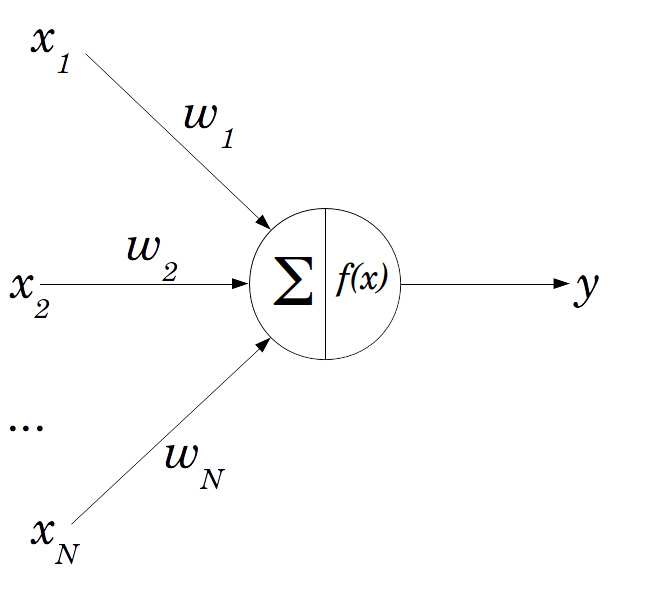
\includegraphics[width=0.325\textwidth]{perp.jpg}
  \end{center}
\end{wrapfigure}

$$ f(x) = \vec{x} \cdot \vec{w} + b $$ 
\[
y = 
\begin{cases}
    1 & \text{if } f(x) > 0 \\
    0 & \text{otherwise}
\end{cases} 
\]

where \vec{x} is the input vector, \vec{w} is the weight matrix of the perceptron, \vec{b} a bias, and \vec{y} the label. To learn the weights and bias, we first initialize the weights to random values. Then we calculate the output of the perceptron using the formula above. Next, we update the weights: 

$$ w_i = w_i + \alpha(d - y)x_{i}$$

where $t$ is the iterative step we are on, $\alpha$ is the learning rate, a user defined constant, and $i$ the feature number. Repeat for all $N$ data points. Repeat all of the above for as many iterations as it takes for the total error to fall below a threshold:
$$\frac{1}{N}\sum_{j=1}^{N}|d_j-y_j(t)| < T$$

\section{Feedforward Neural Networks}
For the single perceptron to work, our data must be linearly separable. However, some functions, such as XOR (see page 2), are not linear. We can address this by apply a non-linear function called an \textbf{activation function} to the output of the perceptron. To get more variety, we can also stack many non-linear perceptions together, forming a \textbf{feedforward neural network}.

\begin{figure}[H]
    \begin{center}
        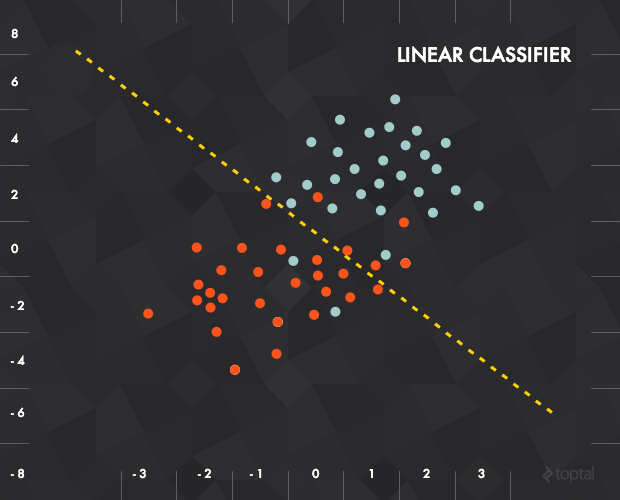
\includegraphics[width=0.4\textwidth]{img1.jpg}
        \hspace{15pt}
        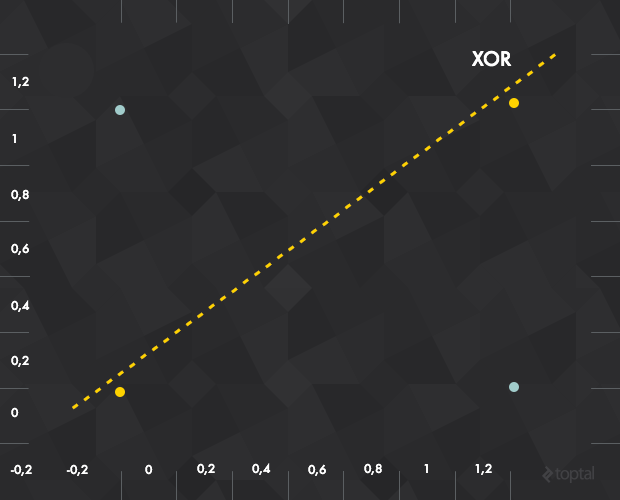
\includegraphics[width=0.4\textwidth]{img2.jpg}
    \end{center}
    \vspace{-10pt}
    \caption{Linear perception classifier and issues with non-linear classification of XOR}
\end{figure}

Now, every perceptron, which we will call a node, can be written mathematically as:

$$ f(x) = \sigma(\vec{x} \cdot \vec{w} + b) $$ 

where $\sigma$ is the activation function. The outputs of $l-1$th layer will serve as $\vec{x_l}$, the input of the $l$th layer. The most common and effective activation function is the ReLU, defined as:

\[
\sigma(x) = 
\begin{cases}
    x & \text{if } x > 0 \\
    0 & \text{otherwise}
\end{cases} 
\]

\begin{figure}[H]
    \begin{center}
        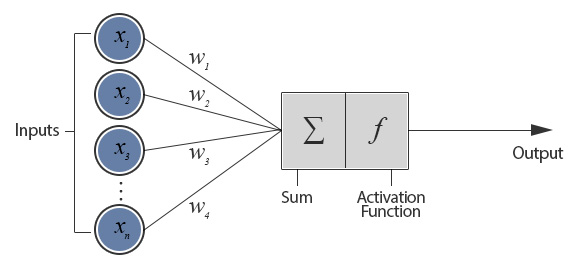
\includegraphics[width=0.475\textwidth]{nnclose.jpg}
        \hspace{15pt}
        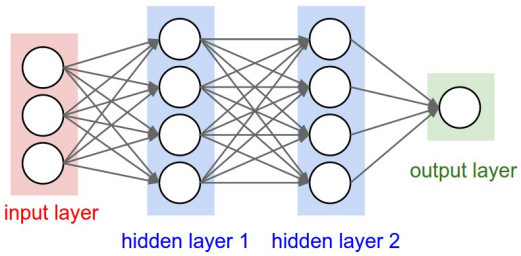
\includegraphics[width=0.4\textwidth]{ffnn.jpg}
    \end{center}
    \vspace{-10pt}
    \caption{Nonlinear perceptron and feed forward neural network}
\end{figure}

\section{Backpropagation Algorithm}
To train our neural network, we rely on the \texbf{backpropagation algorithm}, which incorporates a \textbf{gradient descent} to minimize the error of a neural network on the dataset. Geometrically, this translates to finding the best local minimum in the surrounding region of our initialization in the error graph. For starters, let's define the error function as:

$$ E = \sum_{j}^{N}\frac{1}{2}(y_j-d_j)^2$$

For each weight $w_i$ in the last layer, we want to update it by subtracting the $w_i$ component of gradient multiplied by the learning rate (larger learning rates allow us to skip unfavorable local minimums but also make converging at the bottom of a optimal minimum more difficult):

$$ w_i = w_i - \alpha\frac{\partial E}{\partial w_i} $$

To find the partial for the last layer, we can apply the chain rule.  

$$ \frac{\partial E}{\partial w_i} = (y_j-d_j)*\frac{\partial (\sigma(w_i*x+b))}{\partial w_i} = (y_j-d_j)*\sigma'(w_i*x+b)*\frac{\partial (w_i*x+b)}{\partial w_i}$$

$$ \frac{\partial E}{\partial w_i} = (y_j-d_j)*\sigma'(w_i*x+b)x = \delta_ix$$

For the inner layers, we can write the error as the sum of the errors of the connected nodes in the $l+1$th layer:
$$ E = \sum_{k}^{N_{l+1}}E_k$$

We realize because of the above that we must account for every outgoing weight to each node in layer $l+1$. After doing some math, we end up with:

$$  \frac{\partial E}{\partial w_i} = (\sum_{k}^{N_{l+1}}\delta_k*w_k)*\sigma'(w_i*x+b)*x$$

We can vectorize the above for the complete algorithm machine learning models use. Biases (not vectorized as there is only one per node) are computed in a similar fashion:

$$b_i = b_i - \alpha\delta_i$$

The error function, or \textbf{loss function} as it is more commonly called, be can other functions or a combination of them. For instance, in image restoration, a common technique is to do a weighted sum of the mean square error of the original and reconstructed image and the mean square error of the edge map. One addition to the loss function is a \textbf{regularizer}. In deep learning, we are afraid of overfitting, which can occur if one parameter is too significant and dominates the evaluation. The regularizer will penalize large weights. 

There are other types of tweaks to the basic backpropagation algorithm, called \textbf{optimizers}, such as Adagrad, which adapts the learning rate to individual features, and Adam, which factors in past gradients to calculate current gradients (technique is known as momentum). In Keras, you will be able to specify the optimizer in the fit function. Finally, it is inefficient to backpropagate for every data point, especially if you have tens of thousands of data points. In practice, we train the networks in \textbf{batches}, where we compute a single loss (e.g. average loss) from all data points in the batch. Every iteration of all data points is called an \textbf{epoch}.

\section{Deep networks}
Our neural network layers can be stacked to form very deep neural networks, or deep networks. Research has shown that deeper networks have much better performance, although are more difficult to train. Currently, deep networks of tens or hundreds of layers have beat humans at image classification and can perform tasks ranging from image restoration to natural language processing.

In the following sections, we will give a brief introduction to some advanced types of network architectures, such as convolutional neural networks, which we will be the subject of the next few lectures.

\section{Autoencoders}
Basic feedforward neural networks usually have varied number of nodes per layer. An \textbf{autoencoder} is one that compresses the input and attempts to learn the mapping (the internal structure) to reconstruct the input. Thus, the autoencoder engages in unsupervised learning. the network is split into the encoder stage, where the number of nodes in intermediate layers is always decreasing, to compress the input, and the decoder stage, where the number of nodes is increasing to reconstruct the input. Autoencoders have a limited number of applications, but two prominent ones are image compression and image denoising. 

\begin{figure}[H]
    \begin{center}
        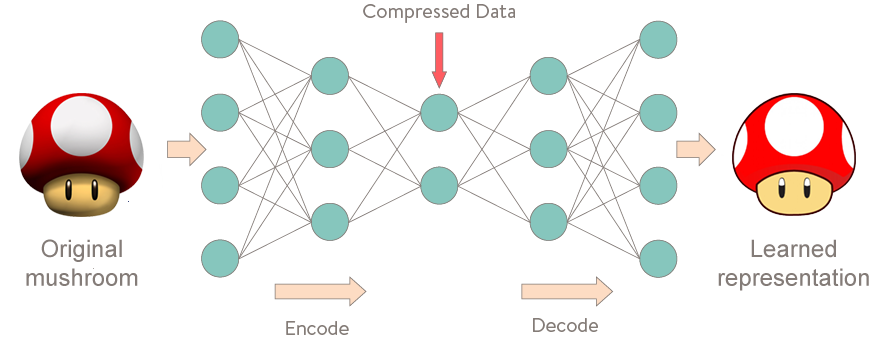
\includegraphics[width=0.8\textwidth]{auto.jpg}
    \end{center}
    \vspace{-10pt}
    \caption{Autoencoders learn to reconstruct the input}
\end{figure}

\section{Convolutional Neural Networks (CNN)}
CNNs are very popular in computer vision, and dominates in image classification and pattern recognition tasks. CNNs are modeled after the animal vision system. Each convolutional block is composed of filters that learn certain image features, which you can think of as forming a 3D block. 

Every filter contains a weight matrix that has the same height, width, and depth of the block before it. The uniformity in depth allows the filter to be convolved with all of the filters before it; when we write the size of the filter, we usually omit the depth as it is already determined. You can think of every filter in a block taking into account every filter in the previous block. As a result, CNNs are known to be computational beasts. We can perform subsampling to reduce the size of the filters at every layer to counter this. Still, without a GPU, it is impossible to train a decent CNN.

\begin{figure}[H]
    \begin{center}
        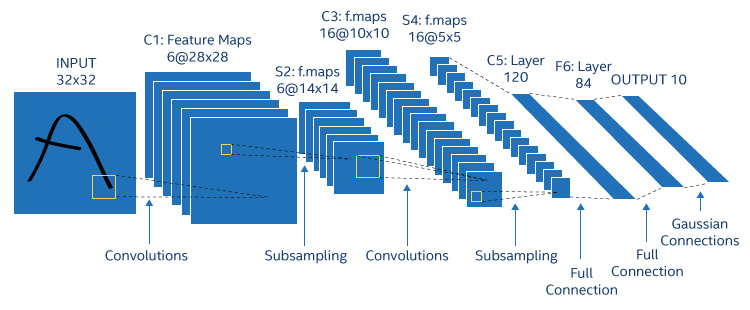
\includegraphics[width=0.95\textwidth]{CNN.jpg}
    \end{center}
    \vspace{-10pt}
    \caption{CNN layout for image classification. Gaussian connectors is a method to classify an image (modern CNNs more commonly use softmax).}
\end{figure}

\section{Recurrent Neural Networks (RNN)}
Traditional neural networks cannot store information from a previous state to be used for the next state. RNNs address this issue by implementing a previous hidden state (the simplest a self-loop) to allow information to persist between states. Figure 6 shows a single RNN block implemented with a self-loop, which gives it the recurrent property. 

\begin{figure}[H]
    \begin{center}
        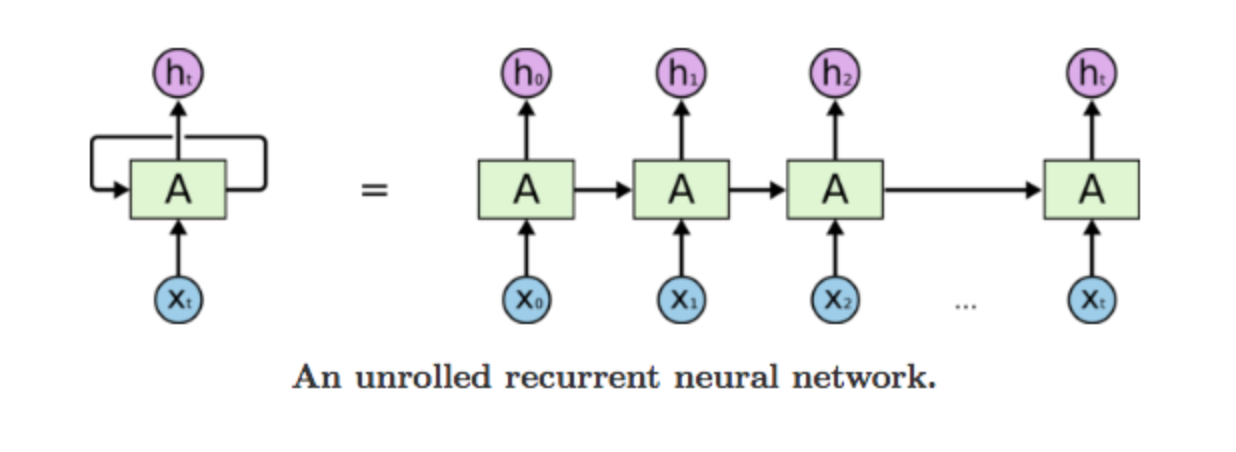
\includegraphics[width=0.8\textwidth]{RNN.jpg}
    \end{center}
    \vspace{-10pt}
    \caption{Consider $x_t$ to be the input and $h_t$ to be the output at state $t$. RNNs allow information from the previous state to be passed to the next state.}
\end{figure}

NNs and CNNs only only input and output of fixed sizes. Recurrent neural networks allow us to have input and output vectors of arbitrary size, and have each element in the vector dependent on the previous elements. To process these sequences RNNs block 'unroll', creating a network with hidden layers across time. This is extremely useful in problems that involve sequences, for instance speech recognition, image captioning, and natural language processing. One example is word generation (many-to-many architecture; see Figure 7). Suppose we have a set of letters and a paragraph composed of the letters. Each input block represents an encoding of the letter and output block contains a softmax classification vector. To generate a word, we select a letter, input it into the RNN, and take the output letter and repeat.

\begin{figure}[H]
    \begin{center}
        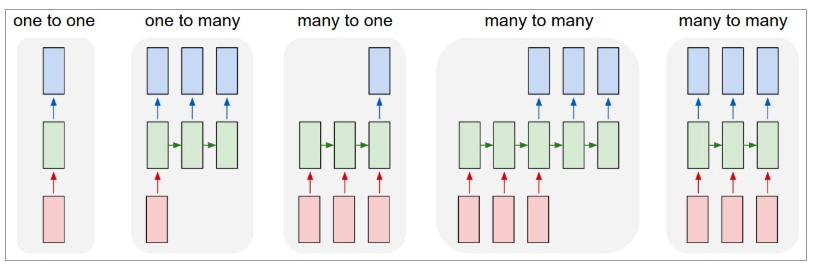
\includegraphics[width=0.6\textwidth]{RNNS.jpg}
    \end{center}
    \vspace{-10pt}
    \caption{Red blocks represent input vectors, green transition states, and blue output vectors.}
\end{figure}

\begin{figure}[H]
    \begin{center}
        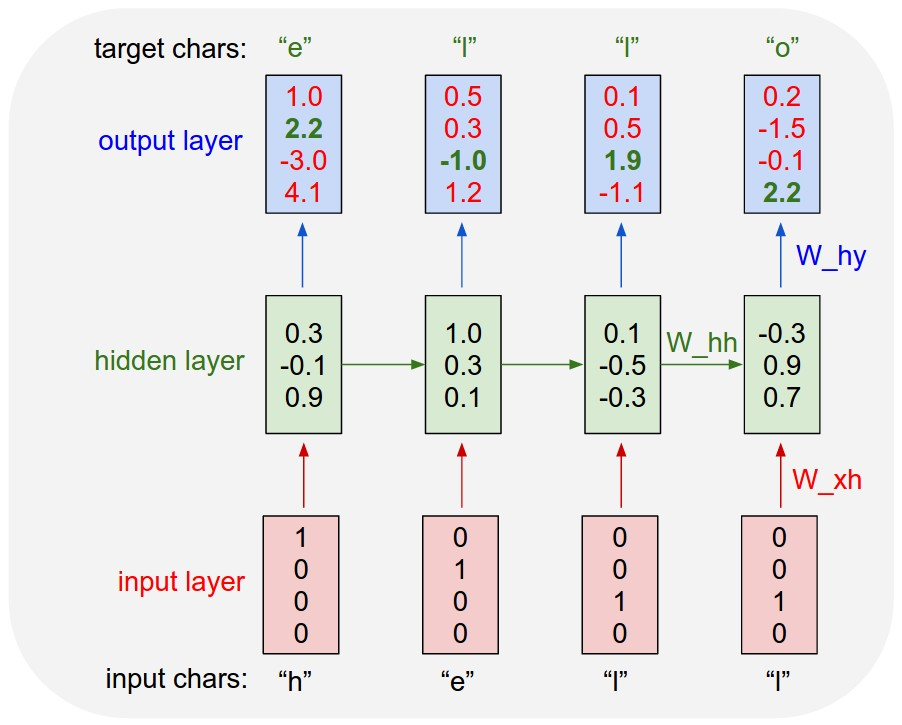
\includegraphics[width=0.4\textwidth]{CLM.jpg}
    \end{center}
    \vspace{-10pt}
    \caption{An example RNN with 4-dimensional input and output layers, and the RNN is unrolled into 4 layers. This diagram shows the activations in the forward pass when the RNN is fed the characters "hell" as input. The output layer contains confidences the RNN assigns for the next character (vocabulary is "h,e,l,o"). We want the green numbers to be high and red numbers to be low.}
\end{figure}

\end{document}